%%%%%%%%%%%%%%%%%%%%%%%%%%%%%%%%%%%%%

%%%%% Disclaimer
%\normalfont
%\begin{frame}
%	\begin{center}
%  		\begin{block}{Disclaimer} 
%The author assumes you know the theory behind Box-Jenkins time series models. \\
%This tutorial will teach you how to apply what you have learned, using R.
%		\end{block}
%	\end{center} 
%\end{frame}

%%%%%%%%%%%%%%%%%%%%%%%%%%%%%%%%%%%%%

%%%%%%%%%%%%%%%%%%%%%%%%%%%%%%%%%%%%%

% Section: Preliminaries

\section[Prelim]{Preliminaries}

% Subsection: Software Installation

\subsection{Software Installation}

%%%%%%%%%%%%%%%%%%%%%%%%%%%%%%%%%%%%%

\begin{frame}
\frametitle{Installing R on a Mac}

\begin{columns}
\column{0.50\textwidth}
\begin{enumerate}
\item Go to \small \ttfamily http://cran.r-project.org/ \normalfont \normalsize and select \itshape MacOS X \normalfont
\item Select to download the latest version: 2.9.1 (2009-06-26)
\item Install and Open.  The R window should look like this:
\end{enumerate}
%
\column{0.50\textwidth}
\begin{center}
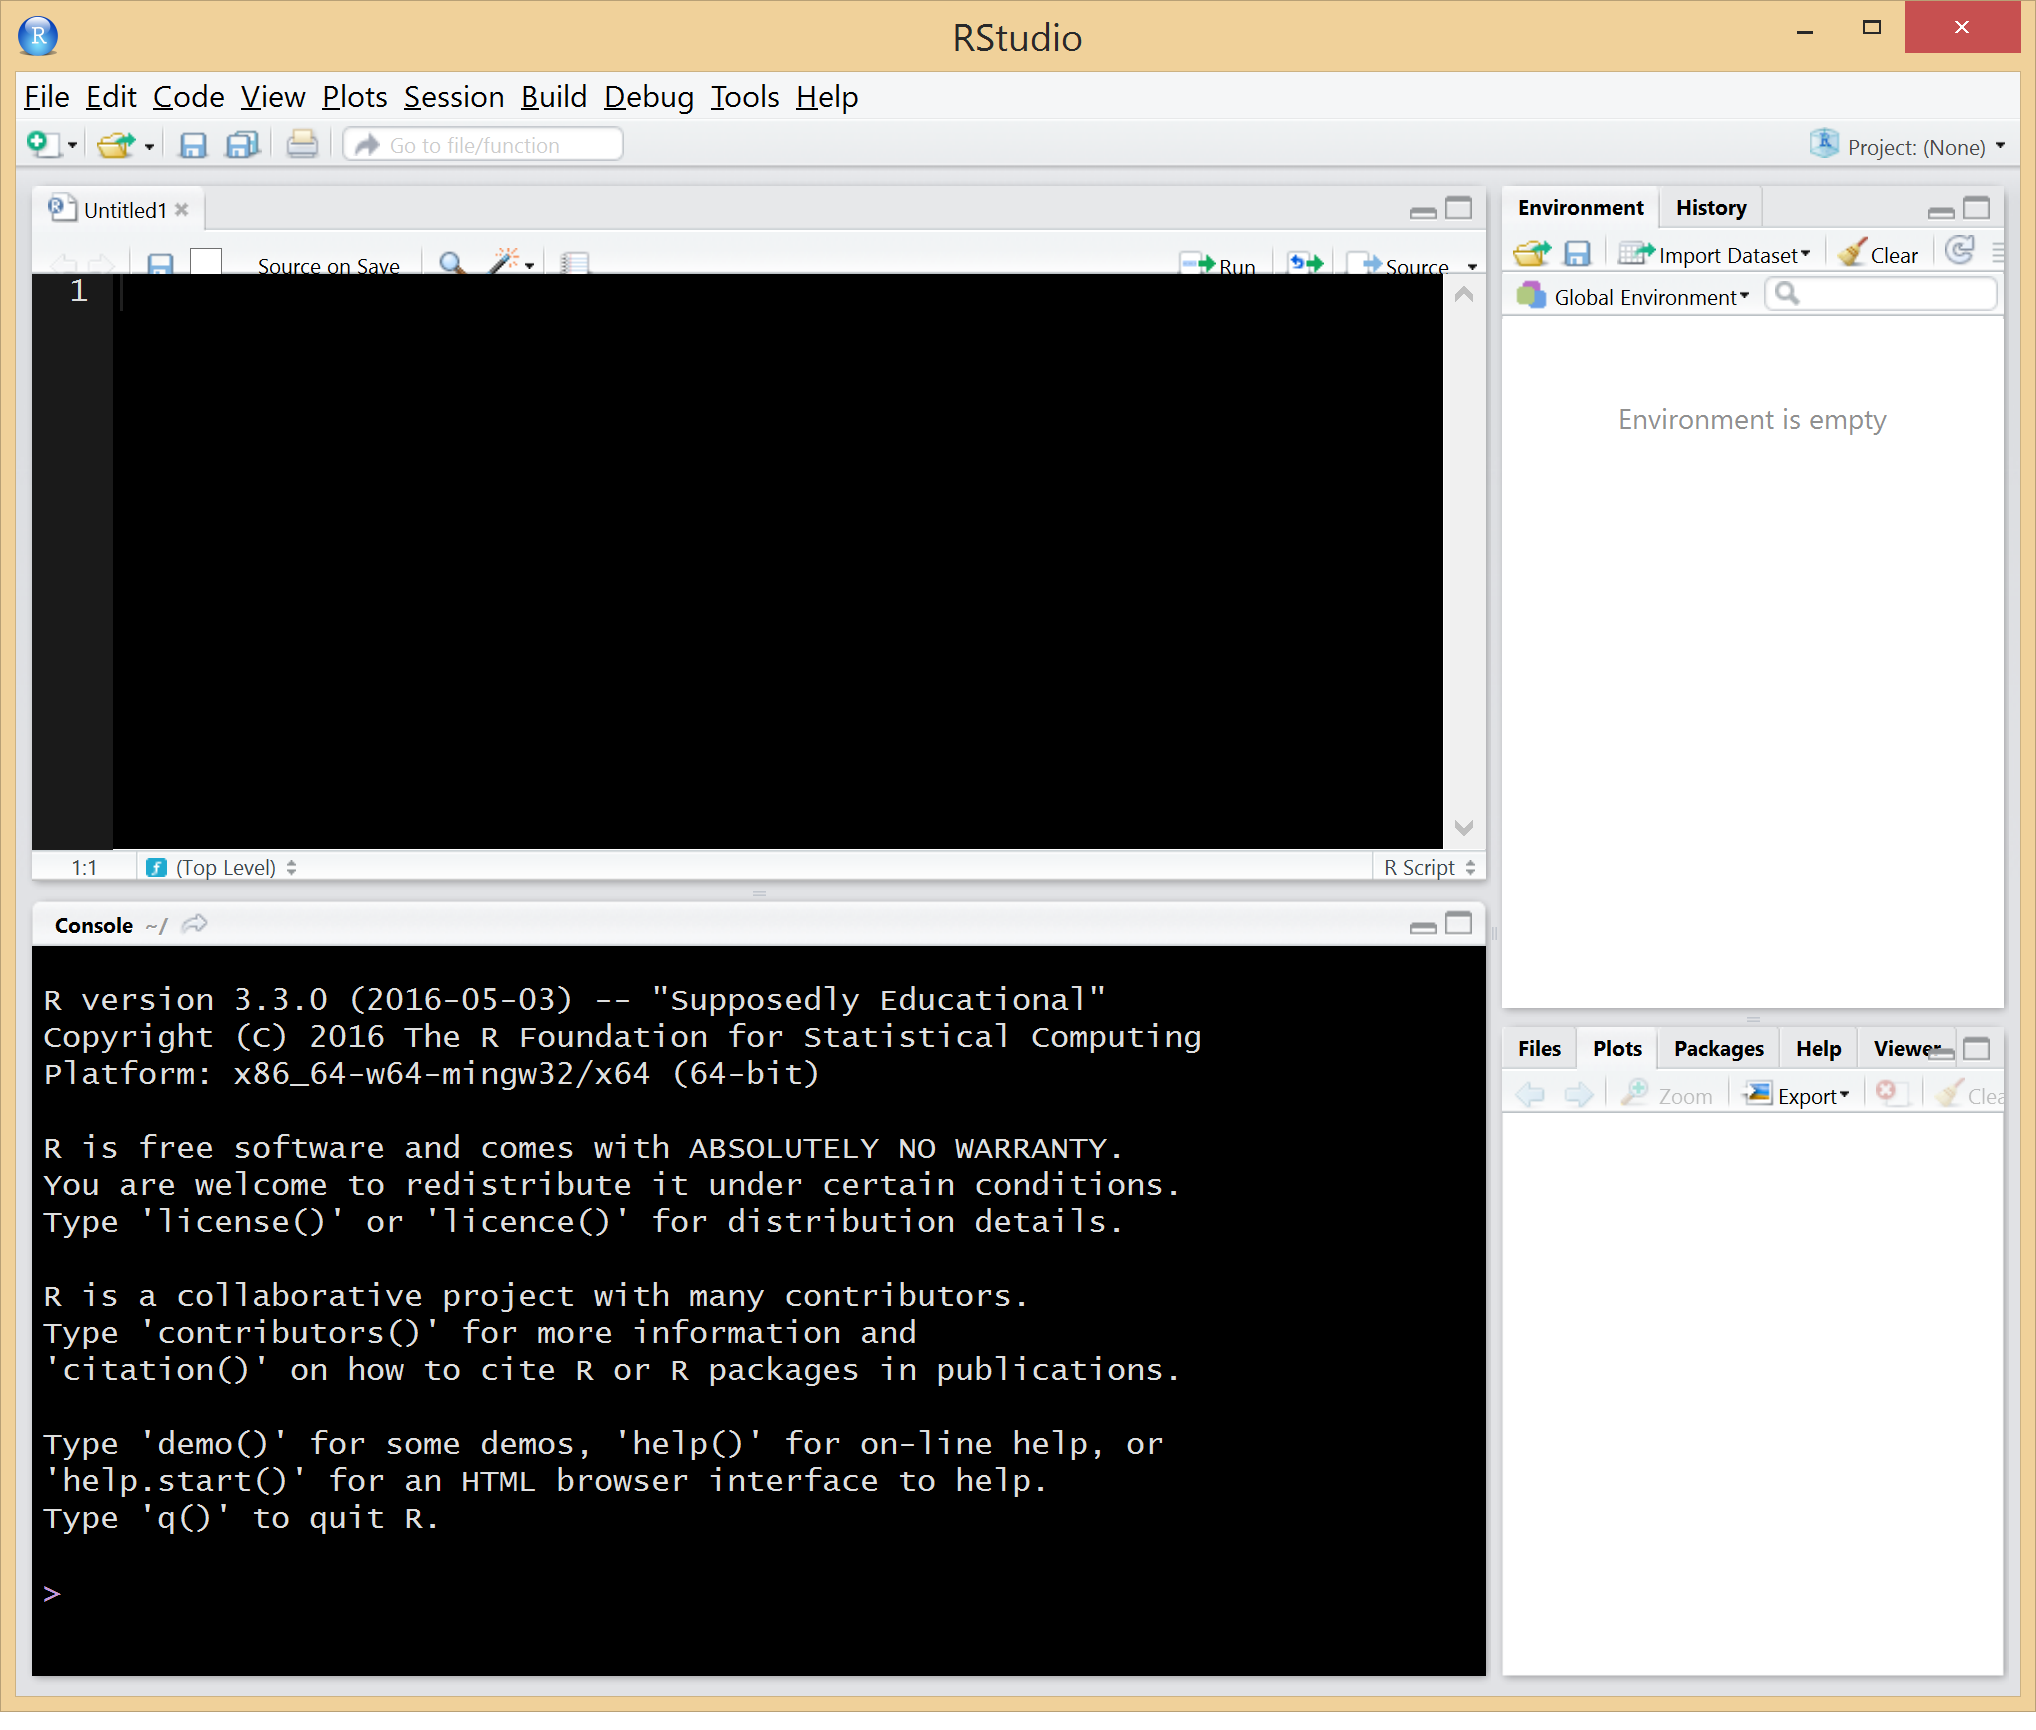
\includegraphics[width=1\textwidth]{images/Rwindow}
\end{center}
\end{columns}

\end{frame}

%%%%%%%%%%%%%%%%%%%%%%%%%%%%%%%%%%%%%

% Subsection: R Help

\subsection{R Help}

%%%%%%%%%%%%%%%%%%%%%%%%%%%%%%%%%%%%%
\begin{frame}[fragile]
\frametitle{R Help}

\begin{columns}
\column{0.4\textwidth}
For help with any function in R, put a question mark before the function name to determine what arguments to use, examples and background information.

\begin{lstlisting}
?plot
\end{lstlisting}

\column{0.6\textwidth}
\begin{center}
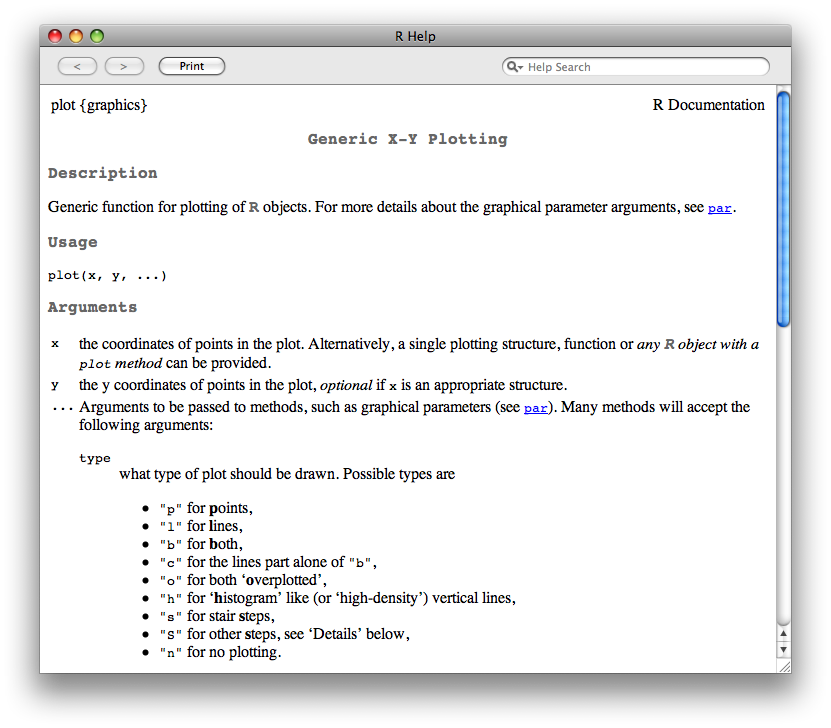
\includegraphics[width=1.1\textwidth]{images/help}
\end{center}
\end{columns}

\end{frame}

%%%%%%%%%%%%%%%%%%%%%%%%%%%%%%%%%%%%%

% Subsection: Importing Data Sets into R

\subsection[Importing Data]{Importing Data Sets into R}

%%% Subsection: Importing Data from the Internet

\subsubsection{Importing Data from the Internet}

%%%%%%%%%%%%%%%%%%%%%%%%%%%%%%%%%%%%%
% --------------------------------------------------- Slide --
\begin{frame}[fragile]
  \frametitle{Data from the Internet}

 When downloading data from the internet, use \ttfamily read.table(). \normalfont  In the arguments of the function:
   \begin{itemize}
   \item \ttfamily header: \normalfont if TRUE, tells R to include variables names when importing
   \item \ttfamily sep: \normalfont tells R how the entires in the data set are separated
     \begin{itemize}
       \item \ttfamily sep=",": \normalfont when entries are separated by COMMAS
       \item \ttfamily sep="$\backslash t$": \normalfont when entries are separated by TAB
       \item \ttfamily sep=" ": \normalfont when entries are separated by SPACE
     \end{itemize}
    \end{itemize}
    	\begin{lstlisting}
data<-read.table("http://www.stat.ucla.edu
/~vlew/stat130a/datasets/twins.csv", 
header=TRUE, sep=",")
	\end{lstlisting}
\normalfont
\normalsize
\end{frame}

%%%%%%%%%%%%%%%%%%%%%%%%%%%%%%%%%%%%%

% Data from your Computer

\subsubsection{Importing Data from Your Computer}

%%%%%%%%%%%%%%%%%%%%%%%%%%%%%%%%%%%%%
\begin{frame}[fragile]
 \frametitle{Importing Data from Your Computer}
     \begin{enumerate}
  	\item Check what folder R is working with now: \\
		\begin{lstlisting}
getwd()
		\end{lstlisting}

  	\item Tell R in what folder the data set is stored (if different from (1)).  Suppose your data set is on your desktop: \\
	\begin{lstlisting}
setwd("~/Desktop")
	\end{lstlisting}

	\item Now use the \ttfamily read.table() \normalfont command to read in the data, substituting the name of the file for the website.
     \end{enumerate}
\end{frame}

%%%%%%%%%%%%%%%%%%%%%%%%%%%%%%%%%%%%%

% Data Available in R
\subsubsection{Using Data Available in R}

%%%%%%%%%%%%%%%%%%%%%%%%%%%%%%%%%%%%%
\begin{frame}[fragile]
  \frametitle{Using Data Available in R}
\begin{enumerate}
\item To use a data set available in one of the R packages, install that package (if needed).

\item Load the package into R, using the \ttfamily library() \normalfont function. \\
	\begin{lstlisting}
library(alr3)
	\end{lstlisting}

\item Extract the data set you want from that package, using the \ttfamily data() \normalfont function.  In our case, the data set is called \ttfamily UN2. \\
	\begin{lstlisting}
data(UN2)
	\end{lstlisting}

\end{enumerate}
\end{frame}

